\section{Fundamentação teórica}

\subsection{Roteadores}
O roteador é o dispositivo responsável por conectar duas ou mais redes ou subredes\cite{kurose}. Ele gerencia todo o tráfego e faz com que vários dispositivos tenham acesso à internet. Alguns tipos de roteadores são: de borda, de distribuição, de núcleo e sem fio.

\subsection{Switches}
O switch é o dispositivo responsável pela conexão física entre servidores, storages e computadores. Os switches são os equipamentos ou softwares responsáveis por organizar e fazer a entrega dos dados, trabalhando como orientadores de tráfego dentro de uma rede. Eles estabelecem a trajetória dos pacotes de dados entre os pontos e como eles se movem de uma área da rede para outra. Esse dispositivo é dividido em 3 tipos, que serão definidos abaixo.

\subsubsection{SWITCH CORE}
Switch core é o termo associado aos comutadores centrais de grandes infraestruturas de TI. Esses equipamentos geralmente são velozes, possuem grande capacidade de comutação de pacotes e várias portas de alta velocidade; por isso, são switches de camada 3.

\subsubsection{SWITCH DE DISTRIBUIÇÃO}
Um switch de distribuição é um componente de rede que atua como ponto de conexão entre os switches de acesso (conectados a dispositivos finais como computadores e impressoras) e os switches de núcleo (ou switches core), que são responsáveis por encaminhar grandes volumes de dados a altas velocidades.

\subsubsection{SWITCH DE ACESSO}

O switch de acesso também é conhecido como switch de borda, pois geralmente está em alguma borda da rede. Ele é conectado a dispositivos operados por usuários finais e, em sua maioria, possui mais portas que os outros switches e tem menor custo.

\subsection{Open Shortest Path First - OSPF}
O Open Shortest Path First (OSPF)\cite{rfc2328} implementa o algoritmo de estado de enlace e utiliza o algoritmo Shortest Path First para o cálculo dos melhores caminhos, também conhecido como Dijkstra.

Um de seus princípios de funcionamento é a utilização do conceito de área, ou seja, a definição de um conjunto de roteadores e redes em que o protocolo de roteamento é implementado. Isso faz com que o projeto de uma rede OSPF divida de forma hierárquica os roteadores nas chamadas áreas, com o intuito de diminuir a complexidade e minimizar a comunicação entre roteadores. Necessariamente deve existir uma área central, chamada de Backbone (Área 0), que deverá atuar como elo de ligação com as demais áreas existentes. A comunicação entre as demais áreas deve ser feita obrigatoriamente através do Backbone. Um exemplo de rede OSPF dividida em áreas é ilustrado na Figura \ref{fig:OSPFArea}.

\begin{figure}[H]
    \centering
    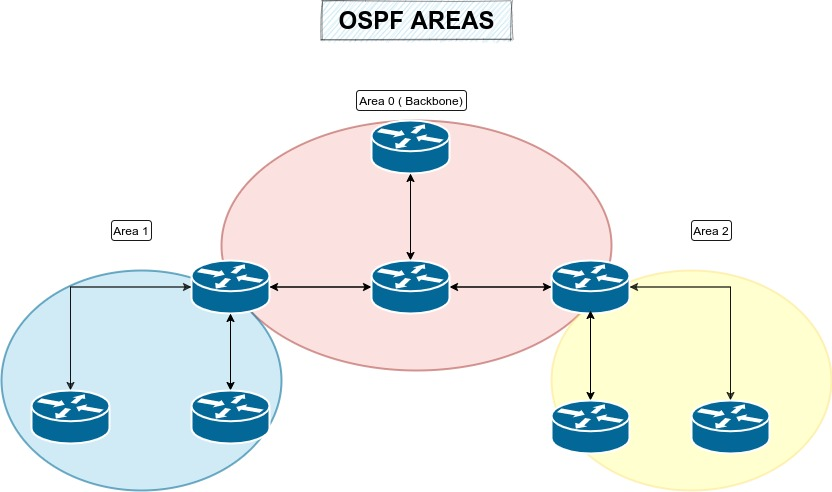
\includegraphics[width=1\linewidth]{fig/OSPFArea.png}
    \caption{OSPF - Áreas}
    \label{fig:OSPFArea}
\end{figure}

Como a figura \ref{fig:OSPFArea} demonstra, uma prática comum, principalmente na área 0, é a ocorrência de roteadores com múltiplas interfaces localizados em diferentes áreas, ou seja, cada interface em uma área diferente. Neste caso, o roteador irá manter uma base de dados da topologia para cada área. Esse é o caso dos roteadores 2, 4 e 7.

O protocolo OSPF funciona utilizando um algoritmo do tipo Link State, o que aumenta a sua complexidade, mas permite uma fácil e eficiente detecção de falhas.

\subsection{VLANS}
Uma VLAN (Virtual Local Area Network ou Rede Local Virtual) é uma tecnologia que permite segmentar uma rede física em várias redes lógicas independentes dentro do mesmo switch. Ela isola o tráfego de dispositivos, aumentando a segurança, o desempenho e facilitando a administração, permitindo agrupar usuários por função, independentemente da localização física.

Cada porta do switch pode ser configurada nas seguintes formas:

\begin{itemize}
    \item Access Port: geralmente são portas conectadas aos dispositivos finais, como PCs, impressoras e servidores.
    \item Trunk Port: normalmente são usadas em uplinks entre switches. Esse tipo de porta transporta frames com a devida identificação de VLAN (tagging), de um switch para outro na rede.
\end{itemize}

A Figura \ref{fig:VLANSMode} representa as seguintes formas de configuração do switch.

\begin{figure}[H]
    \centering
    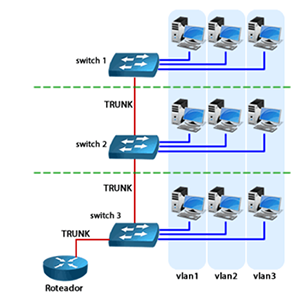
\includegraphics[width=1\linewidth]{fig/VLANSMode.png}
    \caption{Modos de Portas do Switch}
    \label{fig:VLANSMode}
\end{figure}

\subsection{Servidor Web}
O servidor web é um computador que basicamente entrega conteúdo da web para os usuários. Ele faz o armazenamento, processamento e entrega dos arquivos dos sites para os navegadores. Ele também é responsável por processar as requisições de FTP.

\subsection{Network Address Translation}
A Network Address Translation (NAT) \cite{rfc3022} é uma técnica comumente usada por provedores de serviços de internet (ISPs) e organizações para permitir que vários dispositivos compartilhem um único endereço IP público. Ao usar NAT, os dispositivos em uma rede privada podem se comunicar com dispositivos em uma rede pública sem a necessidade de que cada dispositivo tenha seu próprio endereço IP exclusivo.

\subsection{Protocolo Secure Shell - SSH}
O protocolo Secure Shell (SSH) \cite{ssh} é um protocolo para controlar servidores remotamente, gerenciar a infraestrutura e transferir arquivos. Por meio desse protocolo, é possível enviar comandos de forma segura, autenticar e criptografar conexões entre dispositivos.

\subsection{Secure Copy Protocol}
O Secure Copy Protocol (SCP) \cite{scp} é um método baseado no Secure Shell - SSH para transferir arquivos de computador com segurança entre um host local e um host remoto, ou entre dois hosts remotos.

\subsection{Protocolo de transferência de arquivos}

O Protocolo de transferência de arquivos (FTP) é um protocolo de rede padrão usado para a transferência de arquivos de um host para outro em uma rede baseada em TCP, como a Internet \cite{ftp}.

\subsection{Protocolo SNMP}

O \textit{Simple Network Management Protocol} (SNMP) é um protocolo amplamente utilizado para o gerenciamento e monitoramento de dispositivos em redes de computadores. Ele permite que administradores acompanhem o estado e o desempenho de equipamentos como roteadores, switches e servidores de forma centralizada e padronizada \cite{stallings_snmp}.

O funcionamento do SNMP baseia-se em um modelo de comunicação entre um \textit{manager} (gerente) e múltiplos \textit{agents} (agentes). O manager é responsável por solicitar informações ou configurar parâmetros, enquanto os agents são executados nos dispositivos gerenciados e respondem às requisições. As informações são organizadas em uma estrutura hierárquica chamada MIB (\textit{Management Information Base}).

Além das requisições diretas, o SNMP também permite o envio de notificações assíncronas, conhecidas como \textit{traps}, que alertam o manager sobre eventos importantes, como falhas ou mudanças no estado do dispositivo. Isso torna o protocolo essencial para a detecção rápida de problemas e manutenção da qualidade de serviço em redes.

Apesar de sua eficiência e simplicidade, versões mais antigas do SNMP apresentam limitações em relação à segurança. A versão SNMPv3 foi desenvolvida para suprir essas limitações, oferecendo recursos de autenticação e criptografia \cite{rfc3411}.


\subsection{Firewall}

Os firewalls podem ser vistos como barreiras ou gateways que gerenciam o percurso de 
atividades da Web permitidas e proibidas em uma rede privada.  Os firewalls de segurança de 
rede são usados para gerenciamento de tráfego da Web. Normalmente, são destinados a retardar 
a propagação de ameaças da Web.

Para segmentar uma rede são utilizados computadores de gateway especializados chamados de 
roteadores de filtragem. Os firewalls podem ser divididos em:

\begin{itemize}
    \item \textbf{Firewall de rede:} é posicionado na junção entre redes confiáveis e não confiáveis, 
    como sistemas internos e a Internet, Figura \ref{fig:network-firewall}. Sua função principal é monitorar, controlar e decidir sobre a validade do 
    tráfego de entrada e saída com base em um conjunto predefinido de regras. Essas regras foram criadas para 
    impedir o acesso não autorizado e manter a integridade da rede.

    \item \textbf{Firewall baseado em host:} 
    Um firewall de software baseado em host é um software que opera em um único dispositivo dentro de uma rede, 
    Figura \ref{fig:host-based-firewall}.
     Ele é instalado diretamente em computadores ou dispositivos individuais, oferecendo uma camada específica de 
     proteção contra possíveis ameaças. Ao examinar o tráfego de entrada e saída desse dispositivo específico, ele 
     filtra efetivamente o conteúdo nocivo, garantindo que malware, vírus e outras atividades mal-intencionadas não se 
     infiltrem no sistema.
    
\end{itemize}


\begin{figure}[H]
    \centering
    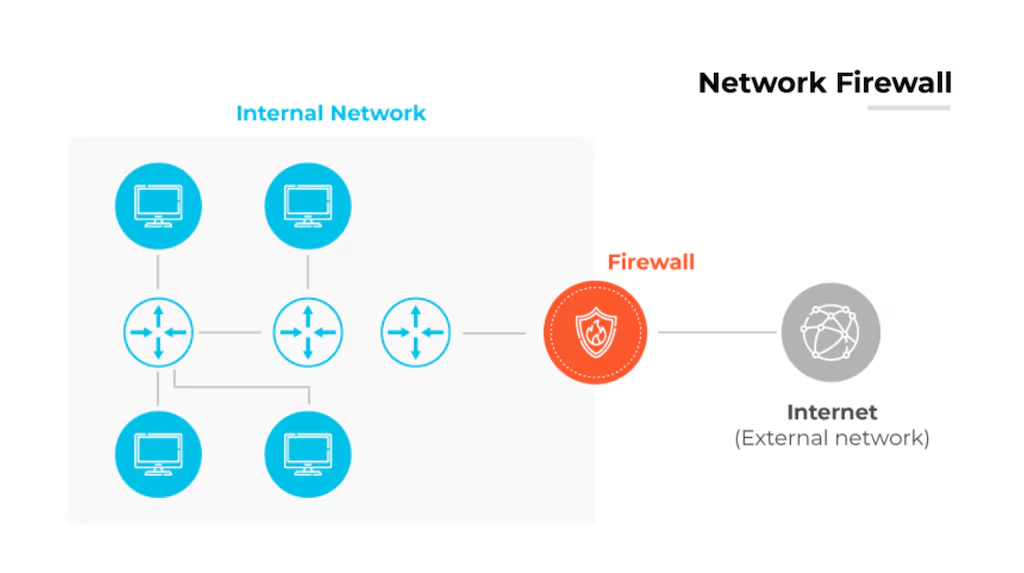
\includegraphics[width=1\linewidth]{fig/network-firewall.png}
    \caption{Firewall de rede}
    \label{fig:network-firewall}
\end{figure}

\begin{figure}[H]
    \centering
    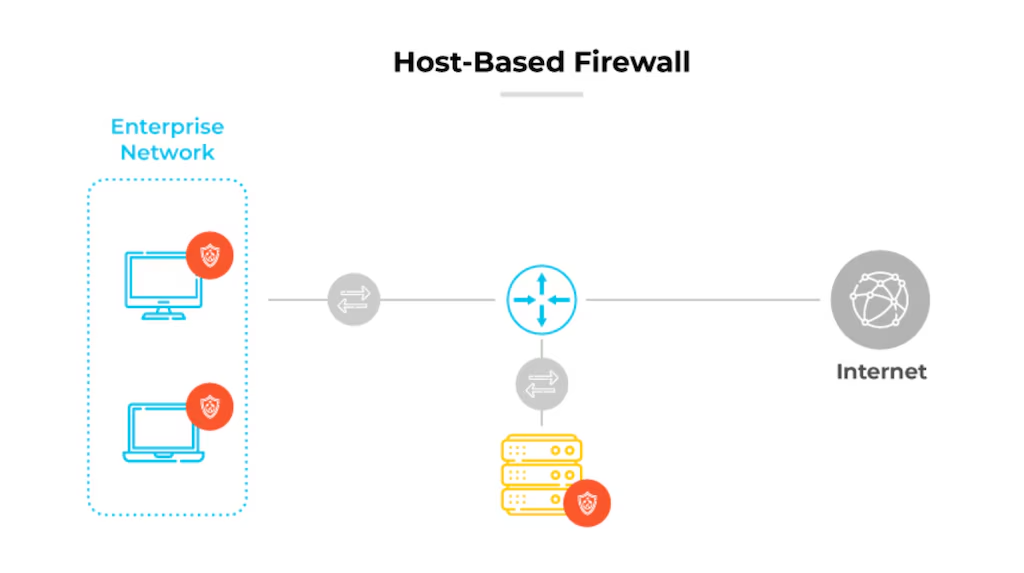
\includegraphics[width=1\linewidth]{fig/host-based-firewall.png}
    \caption{Firewall baseado em host}
    \label{fig:host-based-firewall}
\end{figure}


